\chapter{Principe des Tiroirs}

% \section*{Exemple introductif}
% % Placez ici un exemple motivant illustrant la technique.
%
% \section*{Résumé de la méthode}
% % Résumez ici les idées clés de la méthode avec des repères pour l'élève.
%
% \section*{Exemple applicatif}
% % Un exercice résolu pas à pas montrant l'application de la méthode.
%
% \section*{Exercices guidés}
% % Exercices progressifs
%
%
% \section*{Problèmes complexes}
% % Sélection de problèmes difficiles pour entraîner la maîtrise du chapitre.

\section*{Le principe en quelques mots}
\begin{highlightbox}
    \emph{Si vous placez \( n+1 \) objets dans \( n \) tiroirs, alors au moins un tiroir contiendra plus d’un objet.}
\end{highlightbox}

\begin{center}
    % TikZ - Tiroirs en perspective avec couleur bois et balles 3D
    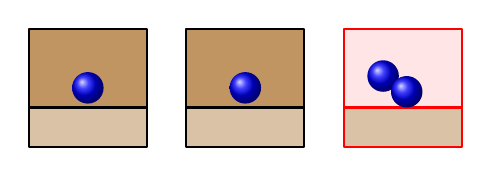
\begin{tikzpicture}[line join=round, line cap=round]

        % Paramètres globaux
        \def\drawerwidth{1.5cm} % Largeur des tiroirs
        \def\drawerheight{1cm} % Hauteur des tiroirs
        \def\depth{0.5cm} % Profondeur (perspective) des tiroirs
        \def\ballradius{0.2cm} % Taille des balles

        % Couleurs personnalisées
        \definecolor{wood}{RGB}{193,154,107} % Couleur bois

        % --- Tiroir 1 ---
        \fill[wood!80!brown] (0,0) -- ++(\drawerwidth,0) -- ++(0,\drawerheight) -- ++(-\drawerwidth,0) -- cycle; % Face avant
        \fill[wood!60!white] (0,0) -- ++(0,-\depth) -- ++(\drawerwidth,0) -- ++(0,\depth); % Dessus
        \draw[thick] (0,0) -- ++(\drawerwidth,0) -- ++(0,\drawerheight) -- ++(-\drawerwidth,0) -- cycle;
        \draw[thick] (0,0) -- ++(0,-\depth) -- ++(\drawerwidth,0) -- ++(0,\depth);

        % --- Tiroir 2 ---
        \begin{scope}[shift={(2,0)}] % Décalage horizontal
        \fill[wood!80!brown] (0,0) -- ++(\drawerwidth,0) -- ++(0,\drawerheight) -- ++(-\drawerwidth,0) -- cycle;
        \fill[wood!60!white] (0,0) -- ++(0,-\depth) -- ++(\drawerwidth,0) -- ++(0,\depth);
        \draw[thick] (0,0) -- ++(\drawerwidth,0) -- ++(0,\drawerheight) -- ++(-\drawerwidth,0) -- cycle;
        \draw[thick] (0,0) -- ++(0,-\depth) -- ++(\drawerwidth,0) -- ++(0,\depth);
        \end{scope}

        % --- Tiroir 3 (en évidence) ---
        \begin{scope}[shift={(4,0)}]
        \fill[wood!80!brown, red!10!white] (0,0) -- ++(\drawerwidth,0) -- ++(0,\drawerheight) -- ++(-\drawerwidth,0) -- cycle; % Face avant avec surbrillance
        \fill[wood!60!white] (0,0) -- ++(0,-\depth) -- ++(\drawerwidth,0) -- ++(0,\depth); % Dessus
        \draw[thick, red] (0,0) -- ++(\drawerwidth,0) -- ++(0,\drawerheight) -- ++(-\drawerwidth,0) -- cycle;
        \draw[thick, red] (0,0) -- ++(0,-\depth) -- ++(\drawerwidth,0) -- ++(0,\depth);
        \end{scope}

        % --- Placement des balles ---
        % Tiroir 1
        \shade[ball color=blue] (0.75,0.25) circle (\ballradius);

        % Tiroir 2
        \shade[ball color=blue] (2.75,0.25) circle (\ballradius);

        % Tiroir 3 (avec deux balles)
        \shade[ball color=blue] (4.5,0.4) circle (\ballradius);
        \shade[ball color=blue] (4.8,0.2) circle (\ballradius);

    \end{tikzpicture}
\end{center}


\section*{Quelques exercices simples}
    \begin{exercise}{Deux personnes du même sexe}
        Parmi trois personnes, il y en a forcément deux du même sexe.
    \end{exercise}

    \begin{exercise}{Anniversaires}
        Parmi 13 personnes, il y en a au moins deux qui sont nées le même mois.
    \end{exercise}

    \begin{exercise}{Cheveux sur la tête}
        Personne n’a plus de 300~000 cheveux sur la tête. Une ville possède 300~001 habitants.
        Peut-on affirmer avec certitude qu’au moins deux personnes ont le même nombre de cheveux sur la tête ?
    \end{exercise}

    \begin{exercise}{Anniversaires multiples}
        Combien de personnes doit-on réunir pour être certain que :
        \begin{itemize}
            \item Deux personnes ont le même anniversaire ?
            \item Trois personnes ont le même anniversaire ?
            \item \( q \) personnes ont le même anniversaire ?
        \end{itemize}
    \end{exercise}
%%%%%%%%%%%%%%

    \begin{exercise}{Perles dans des boîtes}
    Si \( qS + 1 \) perles sont placées dans \( S \) boîtes, alors au moins une boîte contient plus de \( q \) perles.
    \end{exercise}

    \begin{exercise}{Ligne dans un triangle}
    Une ligne \( \ell \) dans le plan du triangle \( ABC \) ne passe par aucun sommet.
    Prouver qu'elle ne peut pas couper les trois côtés du triangle.
    \end{exercise}

    \begin{exercise}{Intersection d’un tétraèdre}
    Un plan ne passe pas par un sommet d’un tétraèdre. Combien d’arêtes peut-il intercepter ?
    \end{exercise}

    \begin{exercise}{Trous sur une cible triangulaire}
        Une cible a la forme d'un triangle équilatéral de côté \( 2 \).
        \begin{itemize}
            \item[(a)] Si elle est touchée \( 5 \) fois, alors il y aura deux trous avec une distance \( \leq 1 \).
            \item[(b)] Si elle est touchée \( 17 \) fois, quelle est la distance maximale possible entre les deux impacts les plus proches ?
        \end{itemize}
    \end{exercise}

    \begin{exercise}{Période d'une fraction}
        La représentation décimale de \( \frac{a}{b} \), où \( a \) et \( b \) sont premiers entre eux, a une période d'au plus \( b - 1 \).
    \end{exercise}

    \begin{exercise}{Décimaux infinis}
        Parmi \( 11 \) décimaux infinis, on peut sélectionner deux nombres \( a, b \) tels que leurs représentations décimales possèdent les mêmes chiffres à une infinité de positions correspondantes.
    \end{exercise}

    \begin{exercise}{Nombres à deux chiffres}
        Parmi \( 12 \) nombres à deux chiffres distincts, on peut en sélectionner deux dont la différence est un nombre de deux chiffre de la forme \( aa \).
    \end{exercise}

    \begin{exercise}{Divisibilité et coprime}
        Si aucun des nombres \( a, a + d, \ldots, a + (n-1)d \) n'est divisible par \( n \), alors \( d \) et \( n \) sont premiers entre eux.
    \end{exercise}
%%%%%%%%%%%

\section*{Quelques exercices}
\begin{exercise}{}
    Parmi \( n+1 \) nombres choisis dans l'ensemble \( \{1, 2, \ldots, 2n\} \), il y en a au moins un qui divise un autre.

    \begin{solution}
        On choisit \( n+1 \) nombres \( a_1, \ldots, a_{n+1} \) que l'on écrit sous la forme \( a_i = 2^k b_i \), où \( b_i \) est impair.
        On a alors \( n+1 \) nombres impairs \( b_1, \ldots, b_{n+1} \) compris dans l'intervalle \( \llbracket 1, 2n-1 \rrbracket \).
        Mais il n'y a que \( n \) nombres impairs dans cet intervalle.
        Donc, deux d'entre eux, \( b_p \) et \( b_q \), sont égaux. Cela implique que l'un des deux nombres \( a_p \) ou \( a_q \) divise l'autre.
    \end{solution}
\end{exercise}

\begin{exercise}
    Soient \( a \) et \( b \in \mathbb{N} \) deux entiers premiers entre eux.
    Alors il existe des entiers naturels \( x \) et \( y \) tels que \( ax - by = 1 \).

    \begin{solution}
        On considère les restes modulo \( b \) des termes de la suite \( a, 2a, \ldots, (b-1)a \).
        Le reste \( 0 \) n'apparaît pas, car \( a \) et \( b \) sont premiers entre eux.
        Si le reste \( 1 \) n'apparaissait pas non plus, alors il existerait deux indices \( p \) et \( q \) tels que \( 0 < p < q < b \) et \( pa \equiv qa \pmod{b} \).
        Cela impliquerait que \( b \mid (q-p)a \).
        Mais comme \( a \) et \( b \) sont premiers entre eux, on aurait \( b \mid q-p \), ce qui est absurde puisque \( 0 < q-p < b \).
        Donc, le reste \( 1 \) apparaît, et il existe un \( x \) tel que \( ax \equiv 1 \pmod{b} \), c'est-à-dire \( ax - by = 1 \).
    \end{solution}
\end{exercise}

\begin{exercise}
Vingt entiers positifs distincts deux à deux sont tous strictement inférieurs à \( 70 \). Montrer que parmi leurs différences deux à deux, il existe au moins quatre valeurs égales.
\end{exercise}

\begin{exercise}
    Soit \( P_1, P_2, \ldots, P_9 \) neuf points de l'espace à coordonnées entières, tels que jamais trois d'entre eux ne soient alignés.
    Prouver qu'il existe un point à coordonnées entières \( L \) situé sur un segment \( P_iP_k \) pour \( i \neq k \).
\end{exercise}

\begin{exercise}
    Soit \( n \) un entier positif qui n'est divisible ni par \( 2 \) ni par \( 5 \).
    Montrer qu'il existe un multiple de \( n \) constitué uniquement de chiffres \( 1 \).
\end{exercise}

\begin{exercise}
    Soient \( a \), \( b \), \( c \) et \( d \) des entiers.
    Montrer que le produit des différences \( b-a \), \( c-a \), \( d-a \), \( c-b \), \( d-b \), et \( d-c \) est divisible par \( 12 \).
\end{exercise}

%%%%%%%%%%%%%%
\section*{Quelques problèmes simples}
% Problème E7 et sa solution
\begin{problem}{Cinq points dans une grille}
    \begin{multicols}{2}
        Cinq points de la grille plane sont choisis.
        Prouvez que vous pouvez toujours en choisir deux tels que le segment reliant ces points passe par un autre point de la grille.
        (Les points de la grille sont ceux qui ont des coordonnées entières.)

        \noindent\resizebox{\linewidth}{!}{%
        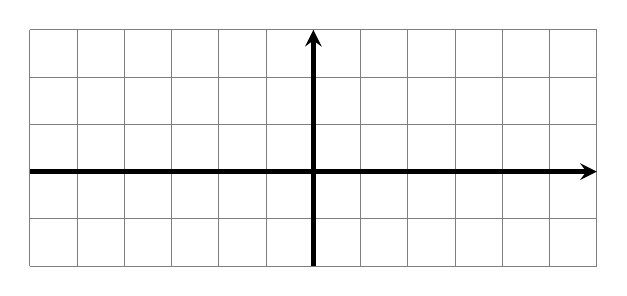
\begin{tikzpicture}[scale=.6, >=stealth]
            \draw[opacity=.5] (-6,-2) grid (6,3);
            \draw[ultra thick, ->] (-6,0) -- (6,0);
            \draw[ultra thick, ->] (0,-2) -- (0,3);
        \end{tikzpicture}}
    \end{multicols}

    \begin{solution}
        Considérons les motifs de parité des coordonnées de ces points de la grille.
        Il n'existe que quatre motifs possibles : (p,p), (p,i), (i,p), (i,i). Parmi les cinq points, il y a nécessairement deux points, notés \( A = (a,b) \) et \( B = (c,d) \), ayant le même motif de parité.

        Considérons le milieu \( L \) du segment \( AB \), donné par :
        \[
        L = \left( \frac{a+c}{2}, \frac{b+d}{2} \right).
        \]
        Puisque \( a \) et \( c \) ainsi que \( b \) et \( d \) ont la même parité, \( L \) a des coordonnées entières, donc c'est un point de la grille.
    \end{solution}
\end{problem}

\begin{problem}{Des gens dans une pièce}
    Il y a \( n \) personnes dans une pièce.
    Montrez qu'il existe au moins deux personnes ayant le même nombre de connaissances dans la pièce.

    \begin{solution}
        Plaçons chaque personne (perle) dans une boîte numérotée \( i \), où \( i \) représente le nombre de connaissances d'une personne. Puisqu'il y a \( n \) personnes et \( n \) boîtes numérotées de \( 0 \) à \( n-1 \), les boîtes \( 0 \) et \( n-1 \) ne peuvent pas être toutes deux occupées.
        Ainsi, il existe au moins une boîte contenant plus d'une perle.
    \end{solution}
\end{problem}

\begin{problem}{Tournoi d'échecs}
    Un joueur d'échecs a 77 jours pour se préparer à un tournoi.
    Il joue au moins une partie par jour, et au total pas plus de 132 parties.
    Montrez qu'il existe une suite de jours consécutifs pendant laquelle il joue exactement 21 parties.

    \begin{solution}
        Soit \( a_i \) le nombre total de parties jouées jusqu'au \( i \)-ème jour inclus.
        Alors, nous avons :
        \[
        1 \leq a_1 < a_2 < \ldots < a_{77} \leq 132 \quad \Rightarrow \quad 22 \leq a_1 + 21 < a_2 + 21 < \ldots < a_{77} + 21 \leq 153.
        \]
        Parmi les 154 nombres \( a_1, \dots, a_{77}, a_1 + 21, \dots, a_{77} + 21 \), il y a nécessairement deux nombres égaux (par le principe des tiroirs).
        Ainsi, il existe des indices \( i \) et \( j \) tels que \( a_i = a_j + 21 \). Cela signifie que le joueur a joué exactement 21 parties pendant les jours consécutifs \( j+1, j+2, \dots, i \).
    \end{solution}
\end{problem}

\begin{problem}{Erdős et Szekeres}
    Les entiers positifs de 1 à 101 sont écrits dans un ordre quelconque. Montrez que l'on peut supprimer 90 de ces nombres, de sorte qu'il reste une sous-suite strictement croissante ou décroissante.

    \begin{solution}
        Nous prouvons une généralisation : Pour \( n \geq (p-1)(q-1) + 1 \), toute suite de \( n \) entiers contient une sous-suite strictement croissante de longueur \( p \) ou une sous-suite strictement décroissante de longueur \( q \).

        Pour tout élément \( m \) de la suite, nous associons \( L_m \), la longueur maximale d'une sous-suite strictement croissante se terminant par \( m \), et \( R_m \), la longueur maximale d'une sous-suite strictement décroissante commençant par \( m \).

        Cette attribution possède la propriété suivante : pour deux éléments distincts \( m \) et \( k \), il est impossible que \( L_m = L_k \) et \( R_m = R_k \). Cela découle du fait que \( m > k \) ou \( m < k \). Les paires \( (L_m, R_m) \), pour \( m = 1, 2, \dots, n \), sont donc distinctes.

        Supposons qu'aucune des sous-suites requises n'existe. Alors, \( L_m \) ne peut prendre que les valeurs \( 1, 2, \dots, p-1 \) et \( R_m \) les valeurs \( 1, 2, \dots, q-1 \). Cela donne \( (p-1)(q-1) \) paires possibles.
        Mais \( n \geq (p-1)(q-1) + 1 \), ce qui contredit le principe des tiroirs.
        \end{solution}
\end{problem}

%%%%%%%%%%%%%%
\section*{Quelques problèmes}
\begin{problem}
    Supposons que $a$ soit premier avec $2$ et $5$.
    Prouvez que, pour tout $n$, il existe une puissance de $a$ se terminant par $\underset{n}{\underbrace{000 \ldots 01}}$.

    \begin{solution}
        Considérons les $10^n$ termes $a, a^2, a^3, \ldots, a^{10^n}$. Prenons leurs restes modulo $10^n$. Le reste $0$ ne peut pas apparaître, car $a$ et $10$ sont premiers entre eux. Ainsi, il y a seulement $(10^n - 1)$ restes possibles :
        \[ 1, 2, 3, \ldots, 10^n - 1. \]

        Par conséquent, deux des termes $a_i, a_k$ (avec $i < k$) auront le même reste, et leur différence sera divisible par $10^n$ :
        \[
        10^n \mid a_k - a_i \iff 10^n \mid a^i (a^{k-i} - 1).
        \]

        Comme $\text{pgcd}(10^n, a^i) = 1$, nous avons $10^n \mid a^{k-i} - 1$, ou $a^{k-i} - 1 = q \cdot 10^n$, ou encore $a^{k-i} = q \cdot 10^n + 1$. Ainsi, $a^{k-i}$ se termine par $000 \ldots 01$ ($n$ chiffres).
    \end{solution}
\end{problem}

\begin{problem}
    Parmi six personnes, il y en a toujours trois qui se connaissent mutuellement ou trois qui sont des étrangers complets.
\end{problem}
\begin{problem}
    Chacun des 17 scientifiques est en correspondance avec tous les autres.
    Ils échangent uniquement sur trois sujets, et chaque paire de scientifiques correspond sur exactement un seul sujet.
    Montrer qu'il existe au moins trois scientifiques qui correspondent entre eux sur un même sujet.
\end{problem}

\begin{problem}
    Parmi dix nombres de deux chiffres distincts, on peut toujours choisir deux sous-ensembles non vides disjoints tels que la somme de leurs éléments soit la même.
\end{problem}

\begin{problem}
    \begin{multicols}{2}
        On place 650 points à l'intérieur d'un cercle de rayon 16.
        Montrer qu'il existe une couronne (un anneau) de rayon intérieur 2 et de rayon extérieur 3 qui contient 10 de ces points.

        \centering
            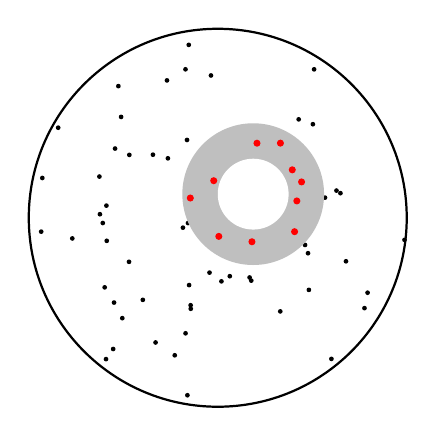
\begin{tikzpicture}[scale=.3]

                % Draw the large circle with radius 16 (scaled down to 4 cm for illustration)
                \draw[thick, fill=white] (0,0) circle (8);

                % Generate random points inside the circle
                \foreach \i in {1,...,75} {
                  \pgfmathsetmacro{\angle}{rand*360} % Random angle
                  \pgfmathsetmacro{\radius}{rand*8}  % Random radius (scaled to 4 for the disk)
                  \fill[black] ({\radius*cos(\angle)},{\radius*sin(\angle)}) circle (0.1);
                }

                % Draw the annular ring (inner radius 2, outer radius 3 scaled down)
                \fill[fill=gray!50!white] (1.5,1) circle (3); % Outer radius (3 scaled)
                \fill[fill=white] (1.5,1) circle (1.5); % Inner radius (2 scaled)

                % Highlight 10 points inside the ring
                \foreach \i in {1,...,10} {
                  \pgfmathsetmacro{\angle}{rand*360} % Random angle within the ring
                  \pgfmathsetmacro{\radius}{2.25 + 0.5*rand} % Random radius between 2 (inner) and 3 (outer)
                  \fill[red] ({1.5+\radius*cos(\angle)},{1+\radius*sin(\angle)}) circle (0.15);
                }

            \end{tikzpicture}

    \end{multicols}
\end{problem}

\begin{problem}
    On dispose de plusieurs cercles, d'une longueur totale égale à 10, placés à l'intérieur d'un carré de côté 1.
    Montrer qu'il existe une droite qui intersecte au moins quatre de ces cercles.
\end{problem}

\begin{problem}
    Une disque fermé de rayon 1 contient sept points, tels que la distance mutuelle entre tous les points est \(\geq 1\).
    Prouvez que le centre du disque est l'un de ces sept points.
\end{problem}

\begin{problem}
    Parmi 70 entiers positifs \(\leq 200\) distincts, montrez que deux d'entre eux ont une différence égale à 4, 5 ou 9.
\end{problem}
